We will now apply the Q-learning algorithm to $L$-Dolinar-receiver calibration problem.

Here, we restrict to $L=2$ processing layers and fix the attenuation coefficients to give equal amplitude at each layer, since the advantage obtained in the success probability is small when optimizing over them as well, see Fig.~\ref{fig:dp_resu}.

The Q-learning algorithm was introduced in Sec.~\ref{ssec:1_rl_qlearning}, and we recall that is consists in exploiting the contractive property of the optimal state-action value function. In our setting, such quantity $Q^*(h_\ell, a_\ell)$ is the average reward that will be enjoyed by the agent, when departing from state $h_\ell$, performing action $a_\ell$, and following the optimal policy afterward. As expected, this quantity reduces to the success probability, as explicitely shown in Sec.~\ref{ssec:optVal}.

Since the $Q$ value is unavailable to the agent, she relies on its estimate $\hat{Q}$, and a tradeoff between exploring and exploiting $greedy$ policies appears, which in Q-learning is tackled by following an $\epsilon$-greedy policy. This consists on choosing, for a given state $h_\ell$, a greedy action with probability $\epsilon$ (\textit{e.g.} the action that maximizes $\hat{Q}(h_\ell, a_\ell)$), or to act randomly with probability $1-\epsilon$.

In contrast to the model-aware case, where the guessing rule was straightforwardly obtained from the Bellman equation at the last time-step, the optimization of state-action value function includes a non-trivial search for the optimal guessing rule, determined by the most likely hypothesis. For a given state $h_\ell$, the agent needs to select a displacement value out of a set $\mathcal{A}(h_\ell)$, which here consists on $21$ points for each displacement, each one ranging from $-1$ to $1$ with step $0.1$, leading to a fairly large state-action space: the agent has $21\times 2 \times 21 \times 2 \times 2=3528$ possible $Q$-values to learn from (including the last guess). We note that each discretized displacement is an independent action or ``button'' in the eyes of the agent ---the agent is dispossessed of any notion of closeness between buttons corresponding to similar values.

In particular, we have studied different schedules for $\epsilon$. While an $\epsilon$ close to 1 will not demonstrate an empirical success rate better than random guesses, an $\epsilon$ value that drops to zero too fast will get stuck in sub-optimal actions (since the agent would not dispose of enough episodes in order to explore the entire state-action space). The update rule for the agent's estimate $\hat{Q}$ is given by Eq.~\eqref{eq:QLUPDATERULE}, with $s_\ell\rightarrow h_\ell$ and learning rates $\lambda_t(h,a)=N_{t}(h,a)^{-1}$ being the inverse of the number of times a state-action pair has been visited. This choice guarantees convergence as per Eq.~\eqref{eq:qLConv}.

As the behaviour of the RL agent strongly depends on the actions chosen at early episodes, we averaged the learning curves over 48 agents. Our results are compared with: \textit{(i)} the maximum success probability attainable with this number of layers and discretization of displacements, Eq.~\eqref{eq:Ldol}, and \textit{(ii)} the success probability attainable via a standard homodyne measurement, which is optimal among Gaussian receivers.

Following our discussion about the figures of merit in Sec.~\ref{ssec:1_rl_bandit}, we have evaluated the performance of our model-free agents at episode $t$ using two figures of merit: \textit{(i)} the cumulative return per episode,
\begin{equation}
\mathbf{R}_{t}=\frac1t\sum_{i=1}^{t}G^{(i)}_{0}=\frac1t\sum_{i=1}^{t}r_{L+1}^{(i)},
\end{equation}
where $r_{L+1}^{(i)}=\{1,0\}$ stands for the correctness of the guess made at episode $i$, and \textit{(ii)} the success probability of the best actions according to the agent, at the current episode,
\begin{equation}
\mathbf{P}_{t}=P_{s}(\alpha,\{a_{\ell}^{(t)*}\}),
\end{equation}
where the best actions $\{ a_{\ell}^{(t)*} \}$ at episode $t$ are obtained by going greedy with respect to the current $Q$-estimate, i.e.,
\begin{eqnarray}
  a_{0}^{(t)*}(h_{0})&=&\argmax{a \in \cA(h_0)} \hat{Q}(h_0,a) \rightarrow h_1^{*} = (o_1, a_0^{(t)*})  \\  \nonumber
  a_{1}^{(t)*}(h^{*}_{1})&=&\argmax{a \in \cA(h^{*}_1)} \hat{Q}(h^{*}_1,a) \rightarrow h_2^{*} = \big( a_0^{(t)*}, o_1, a_1^{(t)*}(h_1^{*}), o_2 \big) \\ \nonumber
  &...& \\ \nonumber
  a_{L}^{(t)*}(h_L^{*}) &=&\argmax{a \in \cA(h^{*}_L)} \hat{Q}(h^{*}_L,a).  \nonumber
\end{eqnarray}
The first figure of merit, $\Rt$, is usually employed to describe the learning process in reinforcement learning, and it evaluates the success rate obtained by the agent so far. On the other hand, the second figure of merit, $\Pt$, is standard in quantum state discrimination, and in our context it evaluates the best strategy discovered by the agent so far. Note that such quantity is unavailable to the agent, but is here used to monitor its learning process.

As $t\rightarrow\infty$, for a \textit{good} learner it is expected that $\Rt\rightarrow\Pt$, \textit{i.e.} with enough agent-environment interactions the average reward should tend to the success probability for the best actions found by the agent, which in turn should converge to the optimal success probability $P_{*}^{(L)}$. Therefore, the learner is not only expected to find a good discrimination strategy, but to also follow it: the interaction policy should tend to the optimal policy. This feature is captured by the evolution of $\Rt$ over different episodes: a good learner is asked to obtain as much reward as possible \textit{during} the learning process.

\begin{figure}[t!]
    \centering
    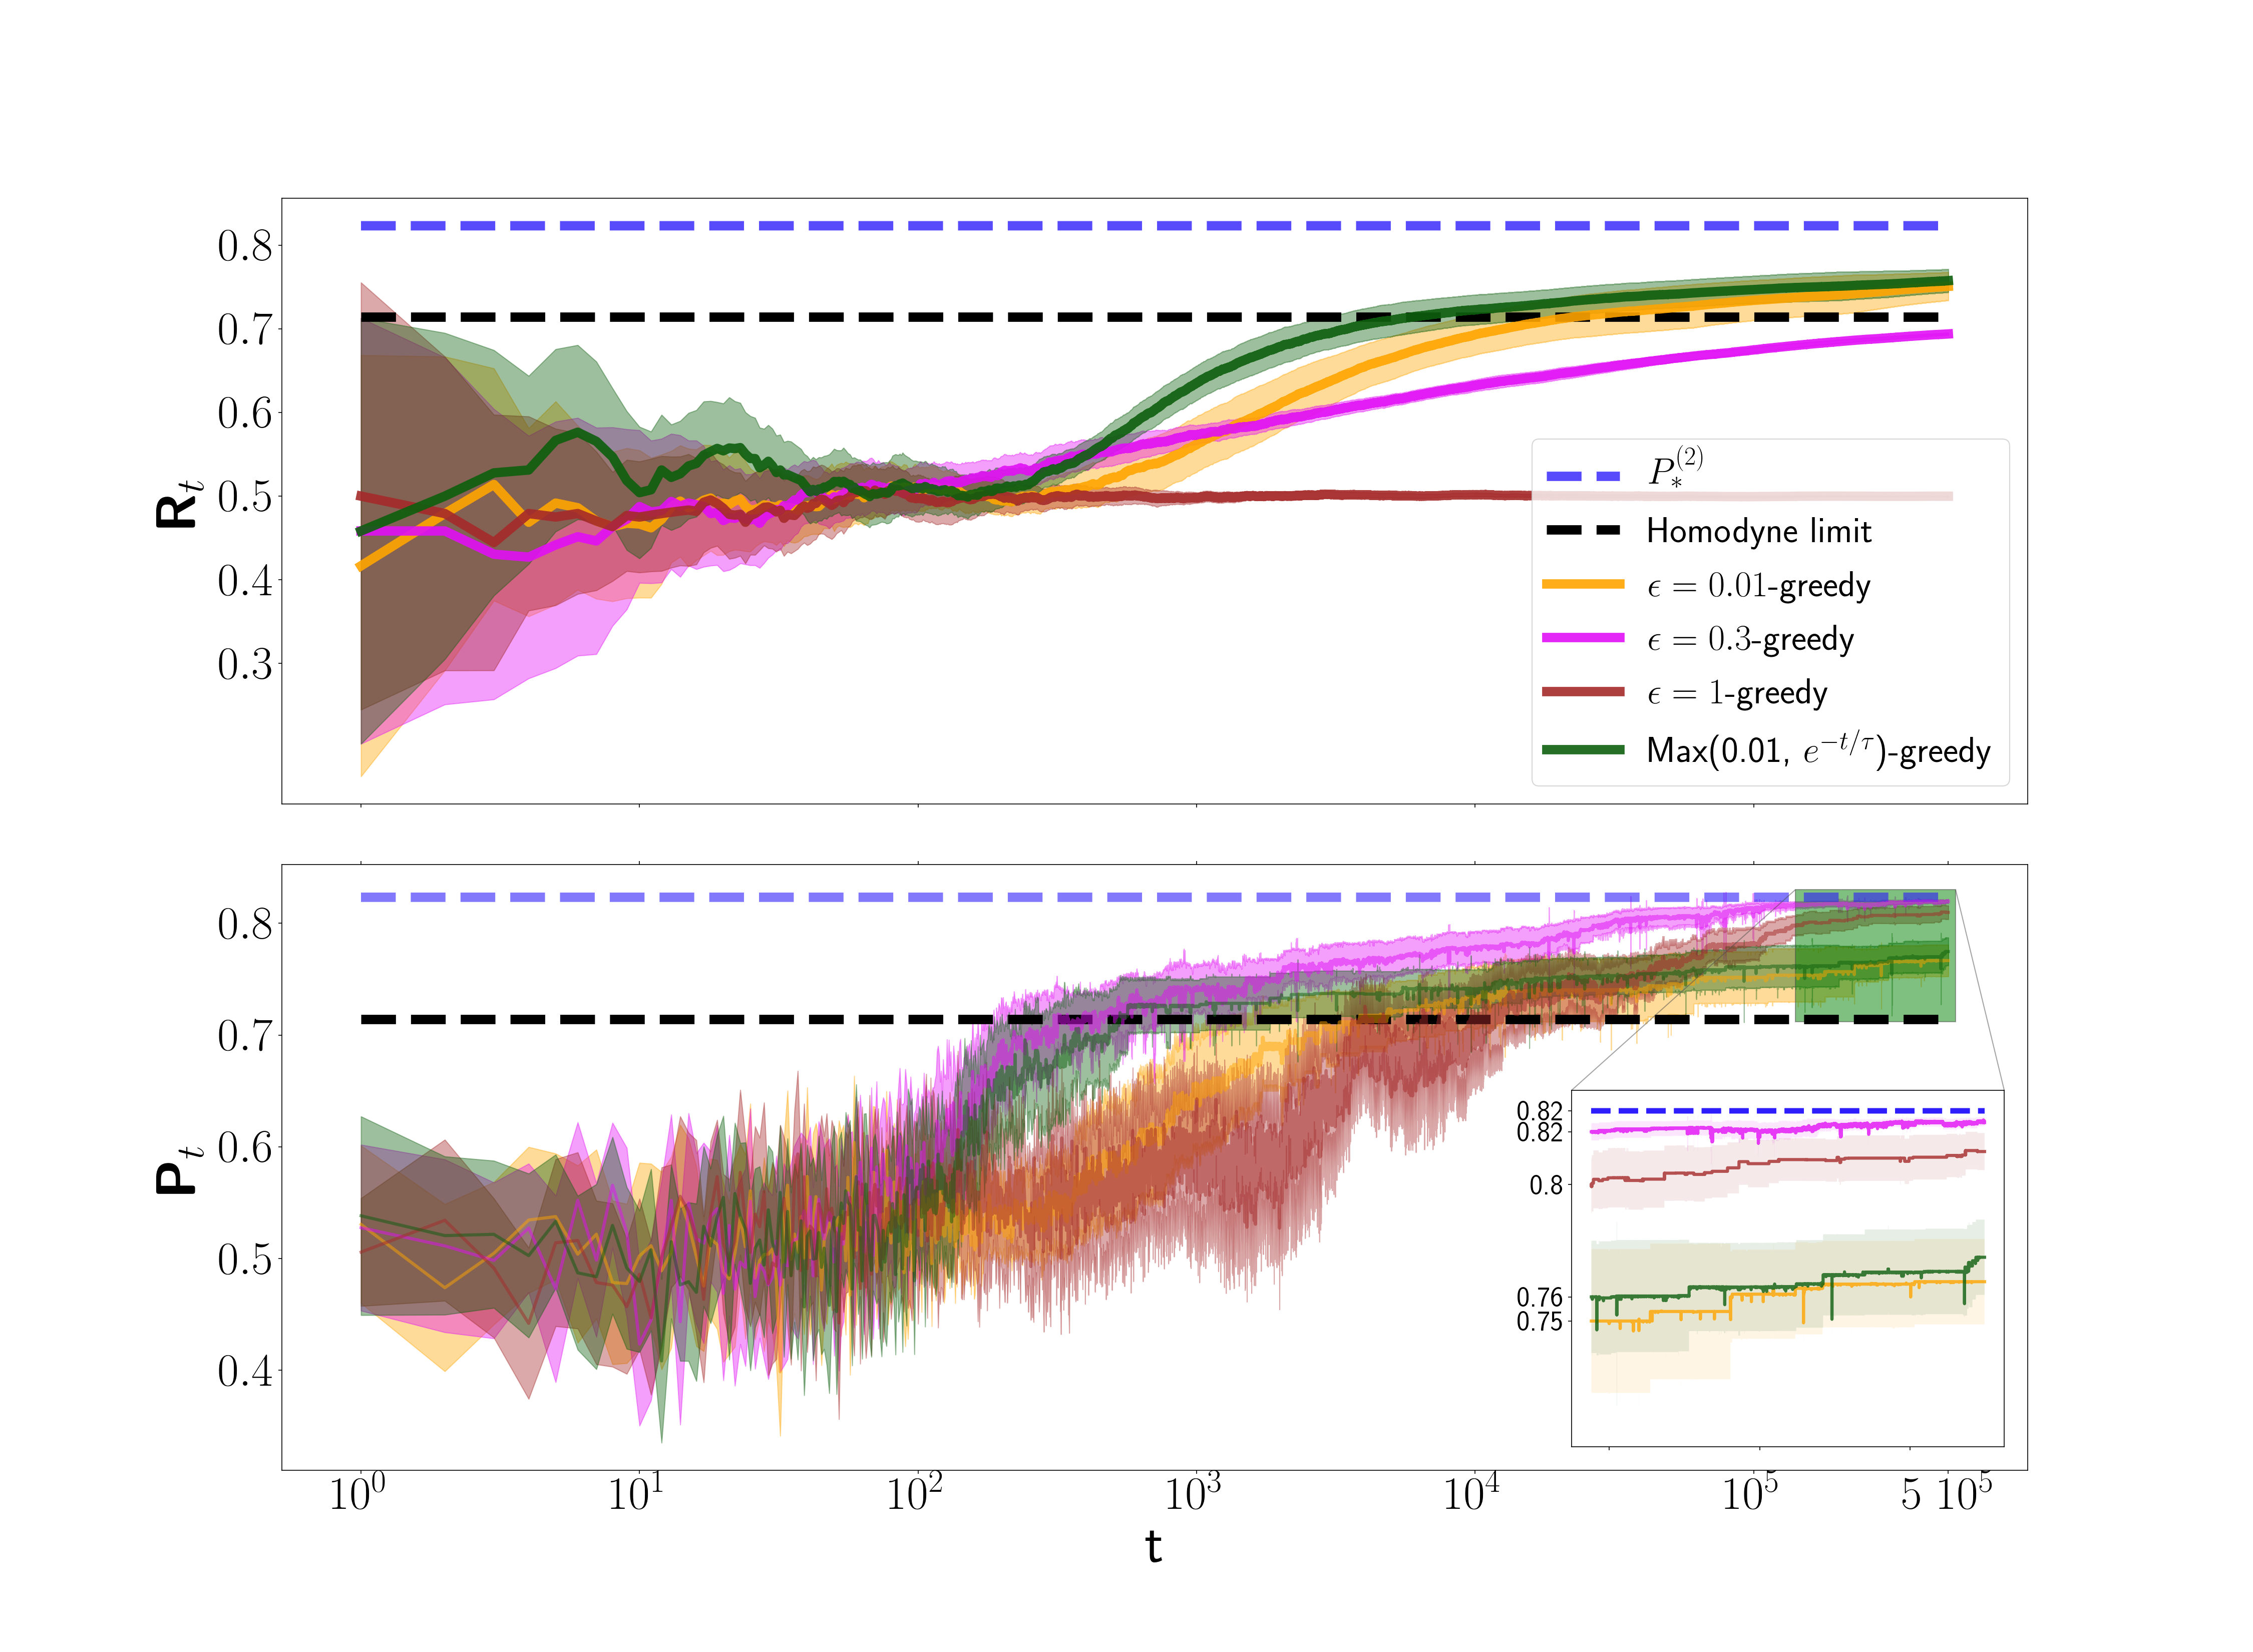
\includegraphics[width=1.\textwidth]{Figures/315/rev_QL.png}
    \caption{We benchmark traditional Q-learning with different \textit{schedules} on $\epsilon$ as the episode number increases. The figures of merit are averaged over $A=48$ agents and show the corresponding uncertainty region. }
    \label{fig:compEpsql}
\end{figure}

In Fig.~\ref{fig:compEpsql} we show the evolution of these two figures of merit for $Q$-learning agents with three different $\epsilon$-greedy interaction policies: \textit{(i)} a completely random one, i.e., $\epsilon=1$, \textit{(ii)} a $0.3$-greedy one, \textit{i.e.}, $\epsilon=0.3$, and \textit{(iii)} a dynamic one (exp-greedy) that becomes exponentially greedier as time passes, \textit{i.e.}, $\epsilon (t)=\max\{e^{- \frac{t}{\tau}},\epsilon_0\}$, with $\epsilon_0=10^{-2}$
\footnote{
This choice assures that at initial episodes the agent favours exploration, whereas at $t = \tau \log \frac{1}{\epsilon_0}$ the agent's behaviour collapses to an $\epsilon_0$-greedy policy.}.

In the first place we note in Fig.~\ref{fig:compEpsql} that, as we mentioned above, a fully random search over the action space ($1$-greedy policy) leads to the extremely poor cumulative reward per episode of $\Rt\approx 1/2$, even for long times, which is expected because a random guess (last action) leads to $P_s(\alpha, \llaves{a_\ell})=1/2$. Instead, since all the actions will be sampled enough times for the agent to learn the optimal policy, $\Pt$  will converge to optimal value at long enough episode number. Nevertheless, if the action space is large, the fully random strategy will require a large number of episodes to explore each action a significant number of times, and for moderate times a $\epsilon$-greedy strategy might reach a better strategy. Indeed, Fig.~\ref{fig:compEpsql} shows that the $0.3$-greedy policy has at all episodes a higher $\Pt$ than the 1-greedy one, being $99\% $ the optimal success probability $P_*^{(L=2)}$ at episode $t=10^{5}$.
Of course, for $0.3$-greedy policy the agent collects many more rewards (actual correct guesses) than for the $1$-greedy  but it is still limited to $\Rt\approx 0.7 P_{*}^{(L=2)}$. In order to reach a better exploration-exploitation trade-off, it is customary to consider an episode-dependent $\epsilon$, e.g. $\epsilon (t)=\max\{e^{-\frac{t}{\tau}},\epsilon_0\}$. Fig.~\ref{fig:compEpsql} shows the results for this tunable interaction policy with $\tau = 2 \cdot  10^{2}$ and $\epsilon_0 = 0.01$.
This allows the agent's $\Rt$ to surpass the homodyne limit at about episode $\sim 5 \cdot 10^{3}$ (which is comparable with the size of the action space), while at later times the performance converges to that of the $0.01$-greedy policy. Note also that $0.3$-greedy discovers a strategy whose $\Pt$ surpasses the homodyne limit at episode $\sim 3 \cdot 10^{2}$.

In Fig.~\ref{fig:315guess} we study the guessing rule discovered by the $0.3$-greedy agent at episode $t= 5 \cdot 10^{5}$. For each sequence of outcomes $o_{1}$, $o_{2}$, we plot the difference between the $Q$-values of guessing for $\ket{-\alpha}$, i.e., $a_{L}=1$, and $\ket{+\alpha}$, i.e., $a_{L}=0$, as a function of the past actions:
\begin{equation}\label{eq:315diff}
\hat{Q} \big( (a_0,o_{1},a_1(h_1),o_{2}),1 \big)-\hat{Q} \big( (a_0,o_{1},a_1(h_1),o_{2}),0 \big).
\end{equation}
Note that the sign of Eq.~\eqref{eq:315diff} corresponds to the agent's best guess for the true hypothesis, since the latter is obtained by going greedy towards $\hat{Q}(h_L,a_L)$, as explained below. We compare these results with the optimal guessing rule in the model-aware setting, plotting a shaded region when the maximum-likelihood guess is $\ket{\pm\alpha}$. The plot shows the agent perfectly learn the guessing rule at the given resolution. Moreover, the difference between the two $Q$-values is more pronounced in the surroundings of the optimal $\beta$ values, meaning that the agents are more confident about their guess in these regions.

\begin{figure}
    \centering
       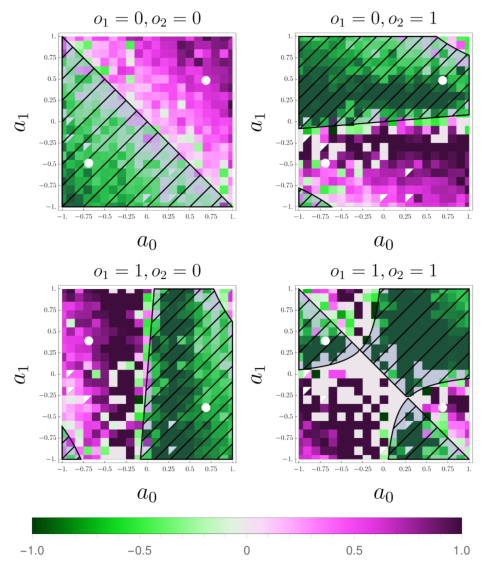
\includegraphics[width=.85\textwidth]{Figures/315/barri.pdf}
    \caption{Density plot of the difference between the estimated $Q$-values for guessing ``plus'' and ``minus'' as a function of the displacements at the first and second layer, for each possible sequence of outcomes, with $\alpha=0.4$. The shaded areas correspond to the regions where the optimal guess, taken according to maximum-likelihood, is ``plus''. The white dots corresponds to the optimal values of the displacements for the proper discretization).
    }
    \label{fig:315guess}
\end{figure}

Our numerical results indicate that standard Q-learning successfully trains agents that surpass the homodyne limit of optical detection and discover strategies whose error rate is comparable with that of the optimal receiver. This is remarkable, especially taking into account that the agents are not initially trained for this task, and run in a model-free setting entirely based on the feedback they get (correct/incorrect) on their guess. While many reinforcement learning schemes focus on extracting the optimal policy from the agent (as measured \textit{e.g.} by $\Pt$), our central figure of merit, $\Rt$, captures the real performance of the agent, and can actually be assessed by the agent itself. It is hence important to design strategies that not only aim at finding the optimal policy within an episode, but also maximize the cumulative reward per episode, reaching $\Rt \rightarrow P_*^{(L)}$ as fast as possible.

As we discussed in Sec.~\ref{ssec:1_rl_bandit}, bandit theory precisely captures such tradeoff by means of the expected cumulative regret. In next sections, we will actually borrow ideas from such a field, in order to enhance the Q-learning agents. Nevertheless, before doing so, let us show how the sequential structure of the receiver is exploited by the Q-learning algortihm.
%
